\chapter{Overview}
\label{vl:tc-overview}

\section{Consortia}
\label{sec:consortia}

Construction of the \dword{dune} detectors is carried out by
``consortia of collaboration institutions'' who assume responsibility
for detector sub-systems.  The consortia plan and
execute the construction, installation and commissioning of their
sub-system.

The \dword{dune} collaboration is pursuing far detector designs based on both
THE single and dual-phase readout technologies currently under
development for \dword{lartpc}. A total
of eleven Far Detector consortia have been formed to cover the
sub-systems required for the two detector types currently under
consideration.  In particular, three consortia (SP-APA, SP-TPC
Electronics and SP-Photon Detection) pursue sub-systems specific to
the single-phase design and another three consortia (DP-CRP, DP-TPC
Electronics and DP-Photon Detection) pursue designs for dual-phase
specific sub-systems.  An additional five consortia (HV System, DAQ,
Cryogenic Instrumentation/Slow Controls, Calibration and Computing)
have responsibility for sub-systems common to both detector
technologies.

Management of the consortia is through an overall Consortium Leader
and a Technical Lead.  The Consortium Leader chairs an institutional
board composed of one representative from each of the collaboration
institutes contributing to the activities of the consortium.  Major
consortia decisions such as technology selections and assignment of
responsibilities within the institutions are expected to be passed
through its Institutional Board.  These decisions are then passed as
recommendation to the \dword{dune} \dword{exb}, described in more detail
below, for formal collaboration approval.

Consortium responsibilities for sub-system deliverables are in many
cases shared by institutions supported by more than one funding
agency.  Each participating funding agency is expected to manage its
own internal project with responsibility for its assigned
deliverables.  Coordination of the separate internal projects
contributing to each consortium is the responsibility of the
consortium Technical Lead.  The Technical lead is responsible for
chairing a consortium Project Management Board incorporating the
separate managers from each of the internal projects that oversees the
inter-connections between the different efforts.

Each consortium is represented on the \dword{dune} \dword{exb} by
its Consortium Leader.  The \dword{dune} \dword{exb} is the primary
collaboration decision-making body and as such includes
representatives from all major areas of activity within the
collaboration.  All collaboration decisions, especially those with
potential impact on the \dword{dune} scientific program or connected with the
assignment of institutional responsibilities, pass through the
\dword{exb}.  \dword{exb} decisions are expected to be
achieved through consensus.  In cases where consensus cannot be
obtained, decision-making responsibility passes to the
co-spokespersons.

\section{Technical Coordination (TCN)}
\label{sec:tc}

Because the consortia operate as self-managed entities, a strong
\dword{tc} organization is required to ensure 
overall integration of the detector elements and successful
execution of the detector construction project.  \dword{tc}
responsibility includes project oversight,
systems engineering, quality assurance and safety.  \dword{tc}
provides support to the Joint Project Office (see
Section~\ref{sec:pm}) for planning and executing the required detector
integration and installation activities in the nearby surface
facilities and underground detector caverns at \surf.

The \dword{tc} organization is shown in Figure~\ref{fig:TC_org_chart}.
\begin{dunefigure}[Organizational chart for \dword{tc}]{fig:TC_org_chart}
  {Organizational chart for \dword{tc}}
  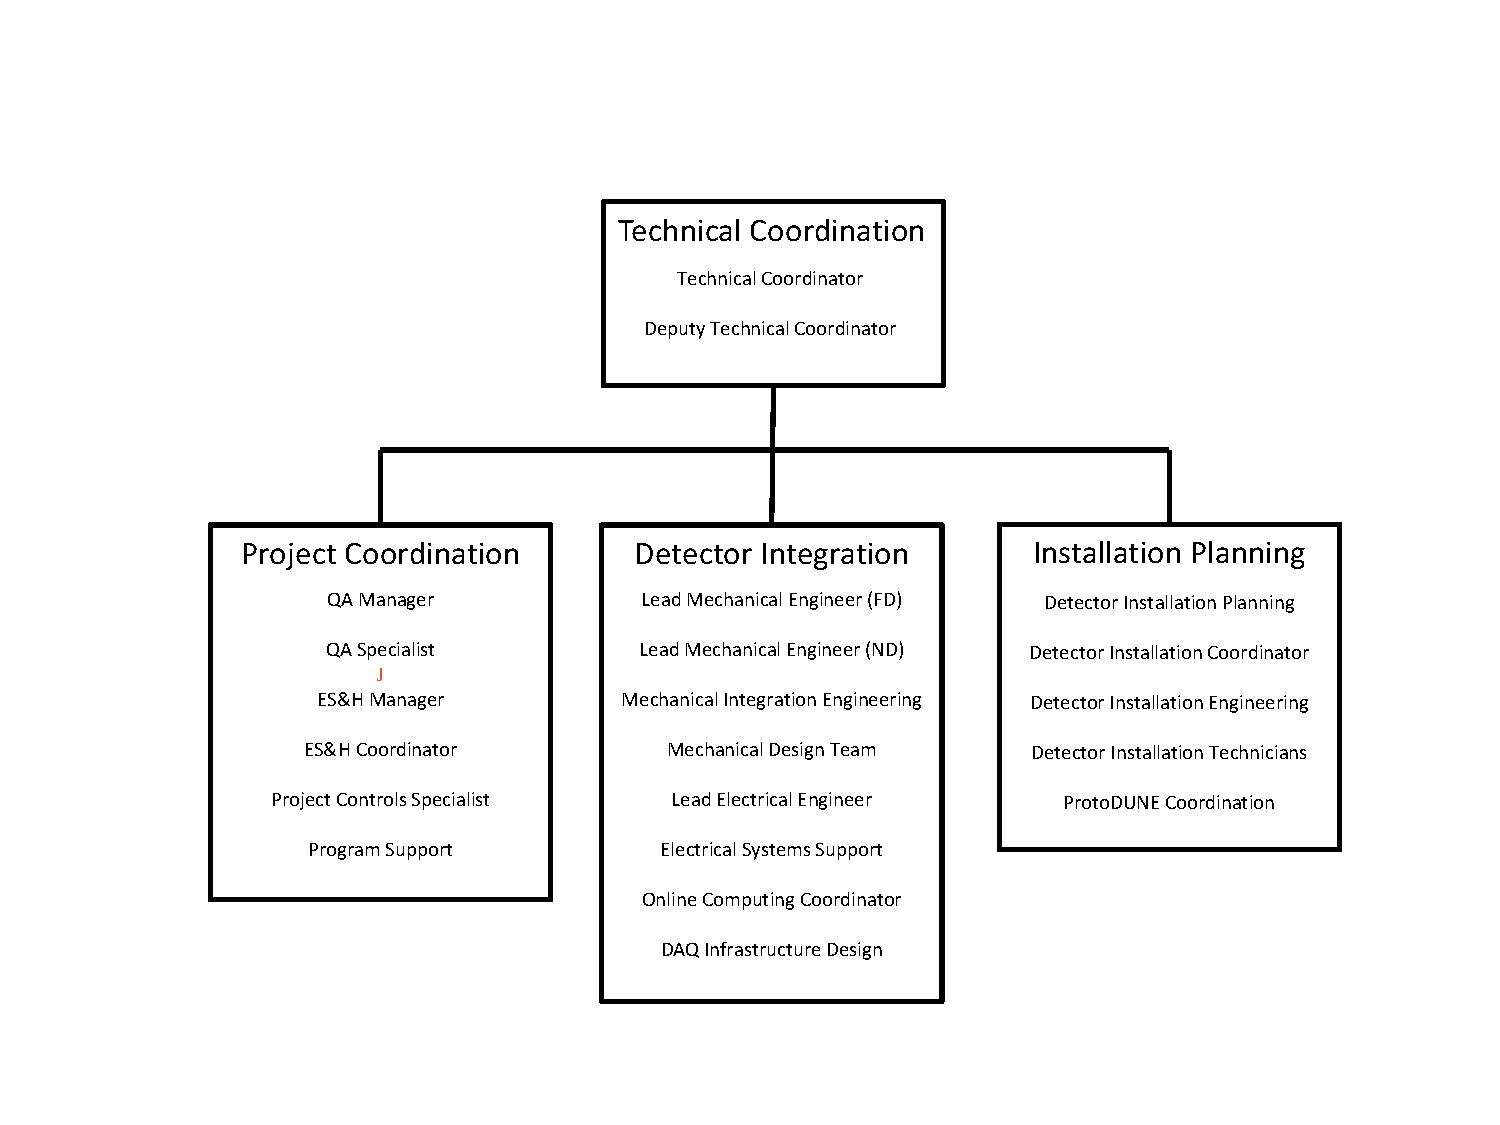
\includegraphics[width=0.75\textwidth]{TC_org_chart.pdf}
\end{dunefigure}
\dword{tc} is headed by the \dword{tcoord}, who is a
Fermilab employee and appointed jointly by the Fermilab Director and
the \dword{dune} Co-spokespersons.  A Deputy Technical Coordinator is
selected from within the collaboration to assist the TC with carrying
out their responsibilities.

The \dword{tc} organization supports the work of the consortia and
takes responsibility for integration of the detector
sub-systems.  The organization includes teams focusing on project
coordination, detector integration and installation support.  The
project coordination team is led by a lead Project Controls
Specialist, a \dword{qa} Manager and an \dword{esh} Manager.  The
detector integration team is directed by a Lead Mechanical and Lead
Electrical Engineer and incorporates an Online Computing Coordinator.
The installation support team is headed by the coordinators for
activities associated with the integration of detector components on
the surface and installation of components in the underground areas.
Each of the three teams incorporates additional personnel that support
these individuals in carrying out their areas of responsibility.

\section{Project Management}
\label{sec:pm}

The \dword{tcoord} manages the overall detector construction
project through regular board meetings with the consortia leadership
teams and members of the \dword{tc} organization.  These
board meetings provide the primary forums for required interactions
between the consortia leadership teams

\dword{tb} meetings are used to evaluate consortia design
decisions with potential impacts on overall detector performance,
ensure that interfaces between the different sub-systems are well
understood and documented, and monitor the overall construction
project to identify and address both technical and interface issues as
they arise.

Project Board Meetings are used to ensure that the scopes of each
consortium are fully documented with assigned institutional
responsibilities, develop and manage risks held within a global
project registry, review and manage project change requests, and
monitor the status of the overall detector construction schedule.

Any decisions generated through these board meetings are passed to the
\dword{dune} \dword{exb} as recommendations for formal approval.
Depending on the specific agenda items to be discussed at these
meetings, the \dword{tcoord} will invite additional members of
the collaboration with specific knowledge or particular expertise to
participate.  In addition, for major decisions, the \dword{tcoord}
will officially appoint three internal collaboration
referees with no direct conflicts of interest to engage in the
process.

\section{Global Project Partners}
\label{sec:partners}

The high level organizational chart for \dword{lbnf} and \dword{dune}
is shown in Figure~\ref{fig:DUNE_org_chart}.
\begin{dunefigure}[Top level organizational chart for \dword{lbnf} and \dword{dune}]{fig:DUNE_org_chart}
  {Top level organizational chart for \dword{lbnf} and \dword{dune}}
  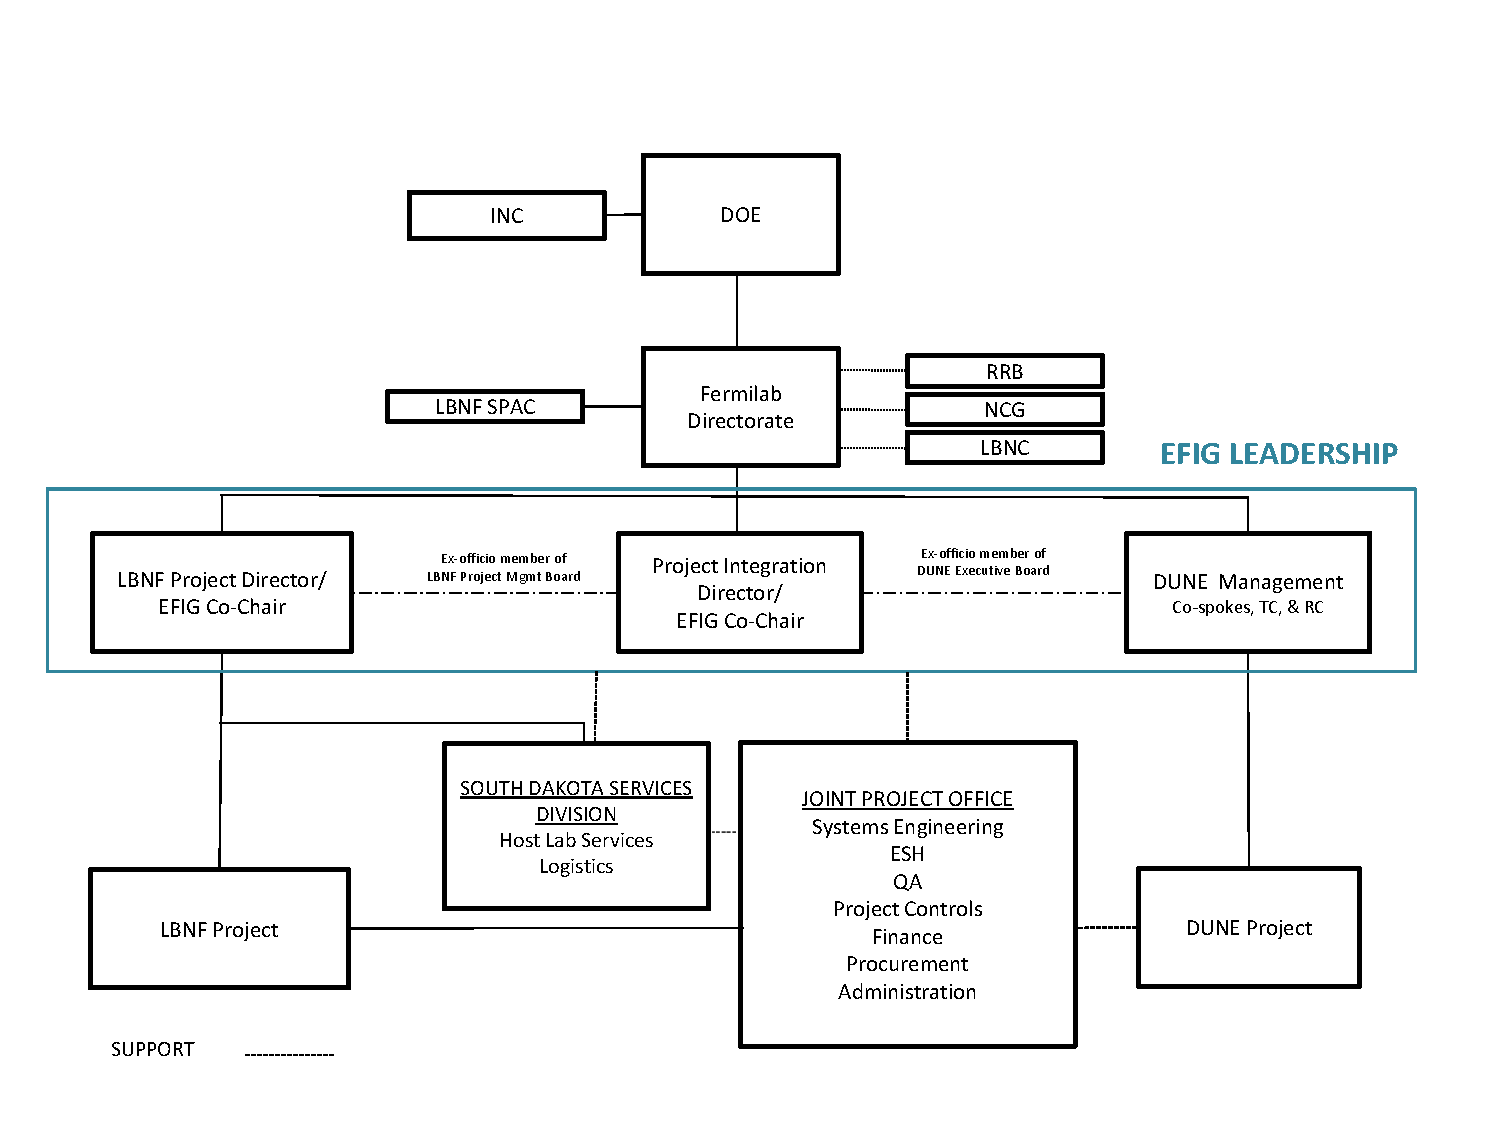
\includegraphics[width=0.95\textwidth]{DUNE_org_chart.pdf}
\end{dunefigure}
The \dword{lbnf} project is responsible for providing conventional
facilities and supporting infrastructure (cryostats and cryogenic
systems) which house the \dword{dune} \dword{fd} modules. \dword{lbnf} is a \dword{us} DOE
project incorporating in-kind contributions from international
partners and is headed by the \dword{lbnf} Project Director who also serves as
the Fermilab Deputy Director for \dword{lbnf}.  Conversely, \dword{dune} is an
international project with some \dword{us} DOE contributions that is
directed by the \dword{dune} collaboration management team.

The Experimental Facilities Interface Group (EFIG) is responsible for
high-level coordination between the \dword{lbnf} and \dword{dune}
projects.  The EFIG is co-chaired by the \dword{lbnf} Project Director and the
Integration Project Director, who is appointed by and reports to the
Fermilab Director and is responsible for the integration and
installation of the detector modules and supporting \dword{lbnf}
infrastructure in the underground areas at \surf post-excavation.  The
Integration Project Director is connected to the facilities and
detector construction projects through their ex-officio positions on
the \dword{lbnf} Project Management Board and \dword{dune} \dword{exb},
respectively.

EFIG leadership incorporates the four members of the \dword{dune}
collaboration management team (co-spokespersons, \dword{tcoord} and
\dword{rcoord}).  The EFIG is responsible for steering the global
project and operates via the consensus.  In the event that an issue
arises for which consensus cannot be achieved, responsibility for
resolving the issue is passed to the Fermilab Director.

The EFIG is supported by a Joint Project Office (JPO) headed by the
Integration Project Director.  JPO functions include global project
configuration and integration, installation planning and coordination,
scheduling, safety assurance, technical review planning and oversight,
development of partner agreements and financial reporting.  The JPO
teams covering each of these areas are formed from the members of the
\dword{lbnf} project and \dword{dune} \dword{tc} teams with
responsibilities towards these same items.  For example, the JPO team
responsible for building the fully integrated model of the detector
within its supporting infrastructure and the surrounding facility
includes members of the \dword{lbnf} Project and \dword{dune} \dword{tc}
teams responsible for integrating the individual elements.

\section{Far Site Integration and Installation}
\label{sec:far_site}

As mentioned previously, the Integration Project Director has
responsibility for the overall planning and execution of activities
associated with component integration and installation both in the
nearby surface facilities and underground detector caverns at \surf.
These activities are necessarily supported by the \dword{dune} consortia who
work with the coordinators of these efforts to develop the overall
plan for assembling and installing the detectors.  The consortia are
also responsible for providing the expert personnel and specialized
equipment necessary to integrate, install and commission their
detector sub-systems.

\dword{dune} \dword{tc} provides support to the core JPO team
responsible for installation planning and coordination.  In
particular, the coordinators and lead technicians associated with the
detector integration and installation efforts are members of the
\dword{tc} organization.  The core team also includes
riggers and other personnel responsible for the transportation and
movement of materials both to and within the SURF facility.  These
team members are associated with the South Dakota Services Division
(SDSD), which is responsible providing host laboratory functions at
the far site.  SDSD members of the JPO core team responsible for
component integration and installation include the rigging teams
responsible for moving materials in and out of the shaft, through the
underground tunnels, and within the detector caverns.  SDSD 
supports team members responsible for safety oversight and logistics
planning at the far site.

The JPO team responsible for installation planning and coordination is
additionally responsible for the specification and procurement of
common infrastructure.  Common infrastructure includes detector pieces
such as racks, cable trays, cryostat flanges, as well as the
mechanical structure that supports the detector components from the
top of the cryostat.  It also includes general items required for
detector integration and installation such as clean rooms, cranes,
scaffolding and personnel lifts. \dword{dune} \dword{tc}
provides engineering resources to the JPO team to support the needed
design efforts. Specialized installation hardware associated with
specific sub-systems is provided by the consortia.

\section{Technical Coordination (TCN) Resources}
\label{sec:tc_resources}

Resources for the personnel and activities associated with \dword{tc}
are provided through a mixture of common collaboration funds and
support from the host nation.  During the construction phase of the
experiment, \dword{dune} will collect an annual membership fee from
each institution based on the number of Ph.D. scientists within the
collaboration.  The collected funds will be used primarily for
supporting the personnel included within the \dword{tc} team.  Funding
agencies will have the option of directly providing team members in
lieu of cash contributions.

The acquisition of common infrastructure will be supported through
additional collaboration common funds collected from the funding
agencies as a percentage of the value of their contributed detector
deliverables.  As in the case above, funding agencies will be given
the option of directly providing equivalently valued infrastructure
items as opposed to actual cash contributions.  Host Laboratory
functions provided by the SDSD will be supported directly host nation
funding agency DOE.

All project partners will sign MOUs that specify which detector
deliverables will be provided by each of the supporting funding
agencies.  The MOU will also specify the required common fund
contributions from each of the participating funding agencies.  The
\dword{dune} resource coordinator will be responsible for managing and
reporting on all common fund contributions.
